\qquad
在过滤栏上输入“ip.addr == 202.117.1.185”过滤掉与认证登录过程不相关的分组,最后确定与TLS协议握手过程相关的分组为第141号分组到第147号分组,如图 \ref{fig6} 所示。点击141号(Client Hello)分组,可以看到该分组中不同网络层的重要字段信息,如图 \ref{fig7} 所示。\\
\begin{figure}
	\centering
	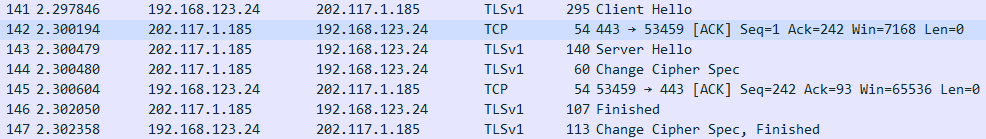
\includegraphics[width=12cm]{image/TLS-1}
	\caption{与TLS握手过程相关的分组}
	\label{fig6}
\end{figure}
\begin{figure}
	\centering
	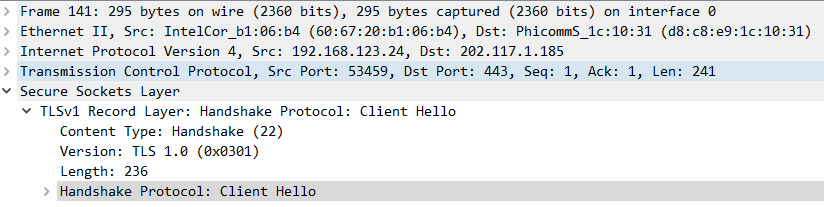
\includegraphics[width=12cm]{image/layer-1}
	\caption{Client Hello分组中不同层次的重要字段}
	\label{fig7}
\end{figure}
\qquad
根据图 \ref{fig7} 反映的分组字段信息,可见最上方的物理层字段反映了分组帧长度为295个字节。被物理层封装的数据链路层,协议为“Ethernet II(第二代以太网)”,显示客户端的设备为“Intel Core(英特尔酷睿系列核心)”,MAC地址为60:67:20:b1:06:b4(十六进制格式);服务端的设备为phi卡,MAC地址为d8:c8:e9:1c:10:31。被数据链路层封装的网络层,协议为IPv4,源地址为192.168.123.24,目标地址为202.117.1.185。被网络层封装的传输层,协议为TCP,源端口为53459,目标端口为443,分组序号(Seq)为1,应答序号(Ack)为1,分组长度为241个字节。重点的SSL(安全传输层)被封装在TCP层中,协议为TLSv1,其中又封装了长度为236个字节的TLS记录层,TLS记录层中又封装了TLS握手协议层,而该握手协议层的握手信息为“Client Hello”。该分组逐层封装的过程体现了计算机网络中的分层思想,将一个分组按类型分为不同的层次有利于逐层分析,简化网络模型。\\
\qquad
和握手协议一样,TLS协议中的更改密码协议也是封装在记录协议中的,通过点击144号分组可以发现这一点,如图 \ref{fig8} 所示。通过观察其他TLS分组的协议结构,验证了记录协议与握手协议、更改密码协议、应用数据协议等其他子协议的层次关系,即这些子协议都封装在记录协议中。\\
\begin{figure}
	\centering
	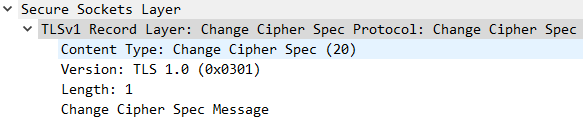
\includegraphics[width=12cm]{image/layer-2}
	\caption{Change Cipher Spec分组中TLS协议层}
	\label{fig8}
\end{figure}
\qquad
根据图 \ref{fig6} 以及各个分组的分层字段信息,可以归纳出本实验中TLS协议握手过程如图 \ref{fig9} 所示。根据图 \ref{fig9} ,TLS协议的握手过程可分为以下步骤:\\
\begin{enumerate}
	\item 客户端向服务端发送Client Hello分组,这组分组包含一段会话编号(Session ID)以及一段随机密钥(如图 \ref{fig10}所示,这是客户端的私钥),期望建立TLS连接,开辟临时会话。
	\item 服务端回复一段TCP应答分组,作为对客户端上一个TCP分组的应答。
	\item 服务端向客户端发送Server Hello分组,这组分组包含一段与Client Hello分组中一致的会话编号(Session ID)和一段随机密钥(如图 \ref{fig11}所示,服务端使用客户端之前发送的私钥给自己的随机密钥加密,这段密钥正是服务端加密后的给客户端共用的公钥),表示同意建立TLS连接,并且接着Server Hello分组的Change Cipher Spec分组中通知客户端使用服务端提供的公钥加密。
	\item 客户端对服务端上一个TCP分组进行应答。
	\item 服务端收到客户端应答后,确认客户端已经知道要使用约定好的公钥加密和解密数据,发送Finished分组期望结束握手。
	\item 客户端收到结束握手分组后,发送Change Cipher Spec分组和Finished分组,表明已完成密钥的更改,结束握手。
\end{enumerate}
\begin{figure}
	\centering
	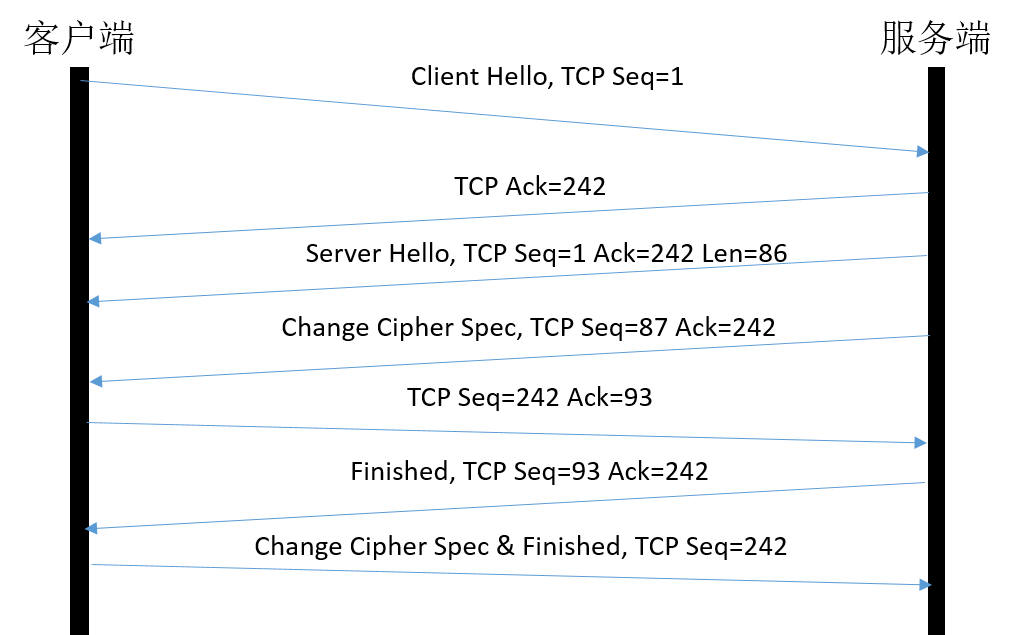
\includegraphics[width=12cm]{image/TLS-Handshake-1}
	\caption{本实验中TLS协议握手过程}
	\label{fig9}
\end{figure}
\begin{figure}
	\centering
	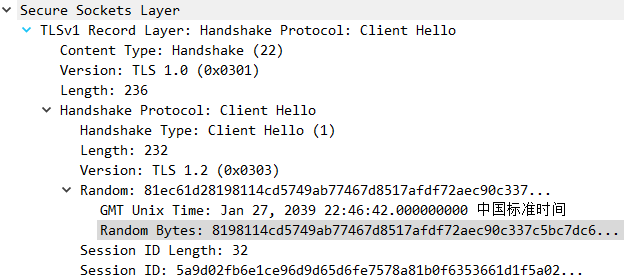
\includegraphics[width=12cm]{image/TLS-Handshake-2}
	\caption{Client Hello分组TLS协议部分}
	\label{fig10}
\end{figure}
\begin{figure}
	\centering
	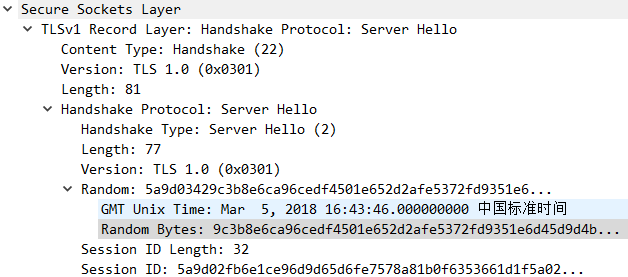
\includegraphics[width=12cm]{image/TLS-Handshake-3}
	\caption{Server Hello分组TLS协议部分}
	\label{fig11}
\end{figure}
\qquad
完成TLS握手后,客户端与服务端的临时会话便使用来自服务端的相同的密钥进行数据的加密和解密,本次临时会话结束后,TLS连接关闭,本次临时会话的密钥无法用于下次会话。以上TLS协议的握手过程说明TLS协议采用面向连接的服务,对应用数据采用对称加密技术。